\documentclass[../main.tex]{subfiles}

\begin{frame}
    \frametitle{IR-Spektrometer}
    \framesubtitle{Was ist es?}
    Analytisches Verfahren, mit dem Molekülstrukturen nachgewiesen werden können
    \begin{itemize}
        \item Infrarotbereich (\SI{3}{\micro\metre}-\SI{8}{\micro\metre})
    \end{itemize}

\end{frame}

\subsection{Komponenten}
\begin{frame}
    \frametitle{IR-Spektrometer}
    \framesubtitle{Komponenten}
    \begin{figure}[ht]
        \centering
        \begin{tikzpicture}
            \node[anchor=south west,inner sep=0] (image) at (0,0) {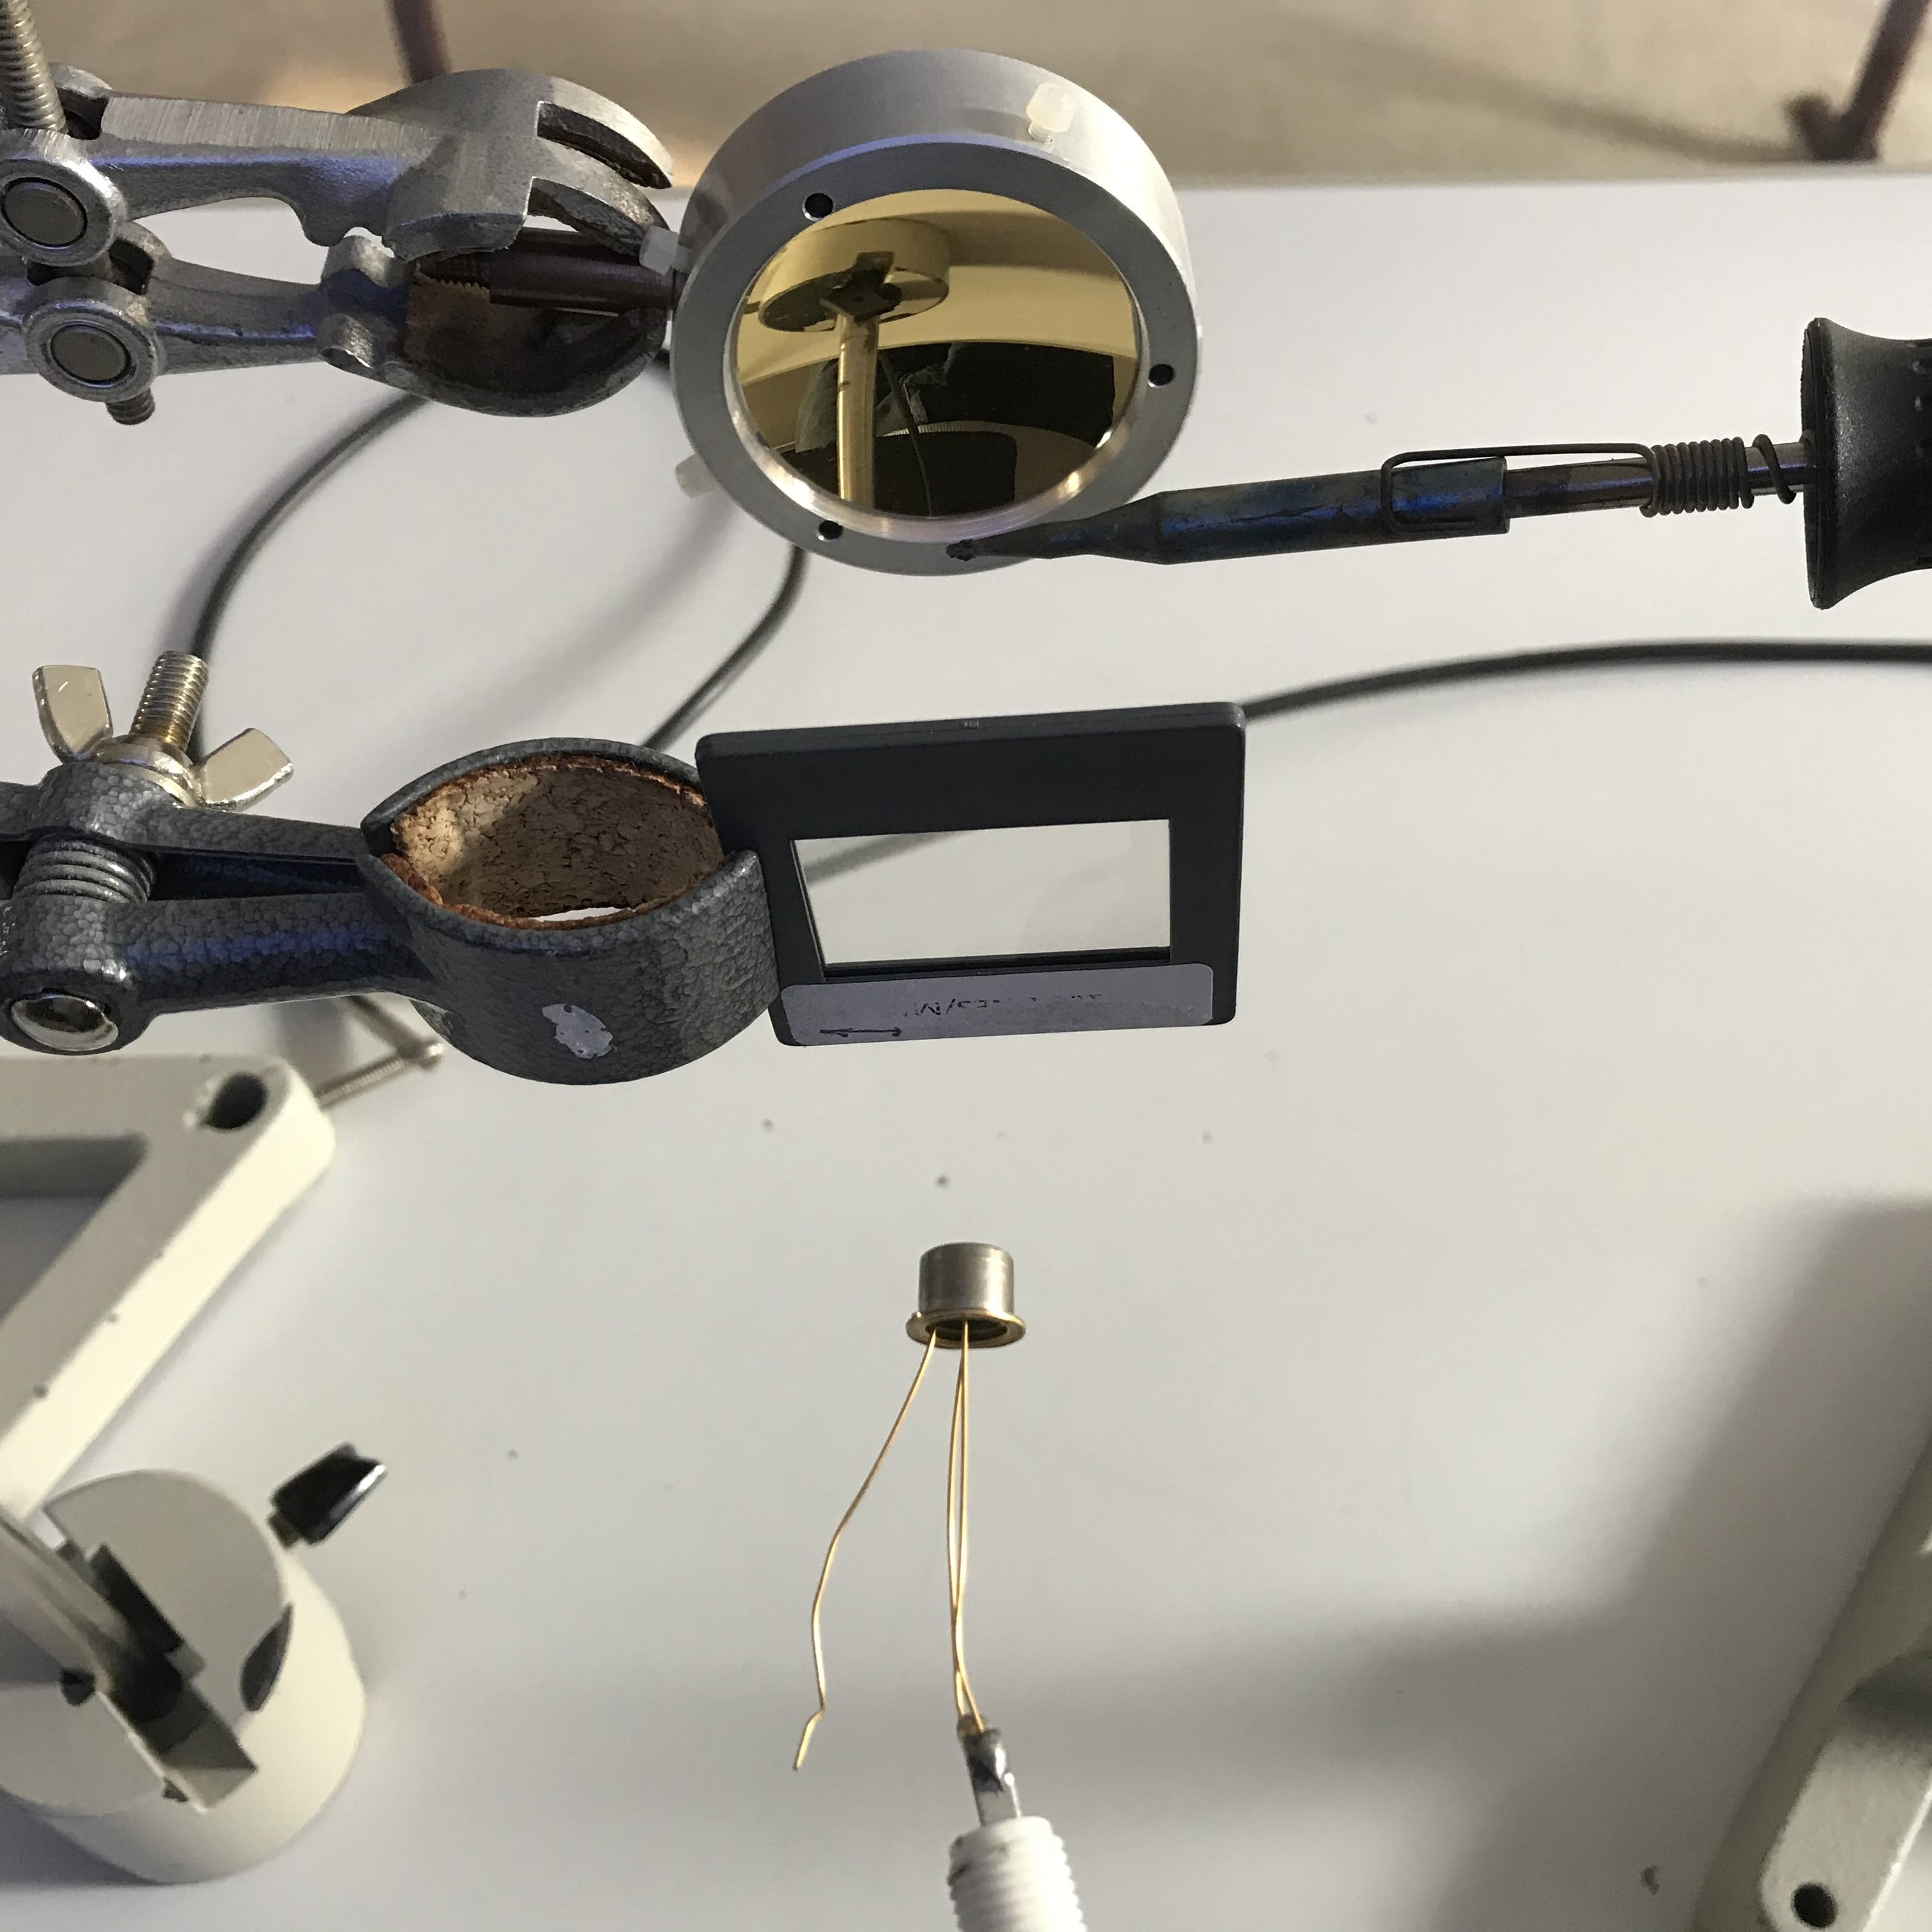
\includegraphics[width=0.6\textwidth]{assets/images/spektrometer-aufbau-frontal.jpg}};
            \begin{scope}[x={(image.south east)},y={(image.north west)}]
                \draw (0.75,0.85) node[fill=white] {Spiegel};
                \draw (0.3,0.7) node[fill=white] {Lötkolben};
                \draw (0.8,0.55) node[fill=white] {Gitter};
                \draw (0.7,0.3) node[fill=white] {Sensor};
            \end{scope}
        \end{tikzpicture}
    \end{figure}
\end{frame}

\begin{frame}
    \frametitle{IR-Spektrometer}
    \framesubtitle{Komponenten}
    Strahlquelle
    \begin{itemize}
        \item Lötkolben
        \item $\lambda_{\text{max}} = \frac{b}{T} = \frac{2.8 * 10^{-3}\SI{}{\metre\kelvin}}{\SI{541}{\kelvin}} \approx \SI{7}{\micro\metre}$
    \end{itemize}
\end{frame}

\begin{frame}
    \frametitle{IR-Spektrometer}
    \framesubtitle{Komponenten}
    Abblendende Optik
    \begin{itemize}
        \item Parabolspiegel
        \item Punktförmiger Strahl $\rightarrow$ Parallelstrahl
    \end{itemize}
\end{frame}

\begin{frame}
    \frametitle{IR-Spektrometer}
    \framesubtitle{Komponenten}
    \begin{columns}
        \column{0.5\textwidth}
        Optisches Gitter
        \begin{itemize}
            \item $b = \frac{k \lambda}{\sin \alpha} = \frac{k \lambda}{\sin \arctan \frac{h}{l}}$
            \item $b_{100} = \frac{\SI{530}{\nano\metre}}{\sin \arctan \frac{\SI{5}{\centi\metre}}{\SI{100}{\centi\metre}}} \approx \SI{11}{\micro\metre}$
            \item Gitter 100 Linien / mm
        \end{itemize}
        \column{0.5\textwidth}
        \begin{figure}
            \begin{tikzpicture}
                \coordinate (max) at (6,6);
                \coordinate (gittermitte) at (3,4);

                % Interference pattern
                \foreach \i in {1,2,...,20}
                    \shade[black,white,shading angle={mod(\i,20)*180}] (6,{\i/4+1.25}) rectangle (6.2,{\i/4+1.5});

                \draw (1,3.75) rectangle (2,4.25);
                \draw (1.5,3.75) node[anchor=north] {Laser};

                \draw[very thick,dashed] (3,3) -- (3,5);
                \draw (3,3) node[anchor=north] {Gitter};
            
                % Sine wave
                \draw[gray,very thin,wavy] (gittermitte) -- (max);
                \draw[blue,ultra thick] (gittermitte) -- (max);
                \draw[gray,very thin,wavy] (2,4) -- (3,4);
                \draw[blue,ultra thick] (2,4) -- (3,4);

                % Labels
                \draw[gray,thick,dashed] (gittermitte) -- (6,4) -- (max) -- (gittermitte);
                \draw (4.5,4) node[anchor=south] {$l$};
                \draw (6,5) node[anchor=east] {$h$};
                \draw (3.5,4) node[anchor=south west] {$\alpha$};
                \draw (6.2,6) node[anchor=west] {$k$};
            \end{tikzpicture}
            \caption{Entstehung von Interferenz am Gitter}
        \end{figure}
    \end{columns}
\end{frame}

\subsection{Versuch}
\begin{frame}
    \frametitle{IR-Spektrometer}
    \framesubtitle{Versuch}
    \begin{columns}
        \column{0.5\textwidth}
        \begin{enumerate}
            \item Lötkolben gibt punktförmigen Strahl ab
            \item Spiegel reflektiert zum Gitter
            \item Gitter beugt Wellen \newline$\rightarrow$ Interferenzmuster
            \item Wellen werden am Sensor dedektiert
        \end{enumerate}
        \column{0.5\textwidth}
        \begin{figure}[ht]
            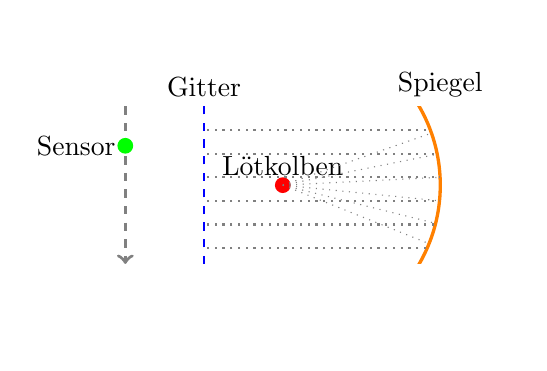
\begin{tikzpicture}
                % Spiegel
                \begin{scope}
                    \clip (2,1) rectangle (4,-1);
                    \draw (1,0)[orange,very thick] circle (2);
                \end{scope}
                \draw (3,1) node[black,anchor=south] {Spiegel};
                
                \fill[red] (1,0) circle (0.1) node[black,anchor=south] {Lötkolben};
                
                % EM-Strahlungen
                \begin{scope}
                    \clip (1,0) circle (2);
                    \clip (0,-1) rectangle (3,1);
                    \foreach \i in {0.3,0.6,...,2} {
                        \draw[gray,dotted] (1,0) -- (3,{\i-1.1}); % Abgegeben
                        \draw[gray,dotted,thick] (4,{\i-1.1}) -- (0,{\i-1.1}); % Reflektiert
                    }
                \end{scope}
                
                \draw[blue,thick,dashed] (0,-1) -- (0,1) node[black,anchor=south] {Gitter};
                
                \draw[very thick,gray,dashed,->] (-1,1) -- (-1,-1);
                \fill[green] (-1,0.5) circle (0.1cm) node[black,anchor=east] {Sensor};
            \end{tikzpicture}
            \caption{Schematischer Versuchsaufbau}
        \end{figure}
    \end{columns}
\end{frame}

\subsection{Ergebnisse}
\begin{frame}
    \frametitle{IR-Spektrometer}
    \framesubtitle{Ergebnisse}
    \begin{figure}[ht]
        \begin{tikzpicture}
            \begin{axis}[
                xmin=0, xmax=150,
                ymin=0, ymax=1023,
                height=0.4\textheight,
                width=\textwidth
            ]
            \end{axis}
            \begin{scope}[x={290},y={100}]
                \draw (0,0) .. controls (0.15,0.25) .. (0.3,0);
                \draw (0.3,0) .. controls (0.45,0.75) .. (0.6,0);
                \draw (0.6,0) .. controls (0.75,0.25) .. (0.9,0);
            \end{scope}
        \end{tikzpicture}
        \caption{Erwartetes Signal}
    \end{figure}
    \begin{figure}[ht]
        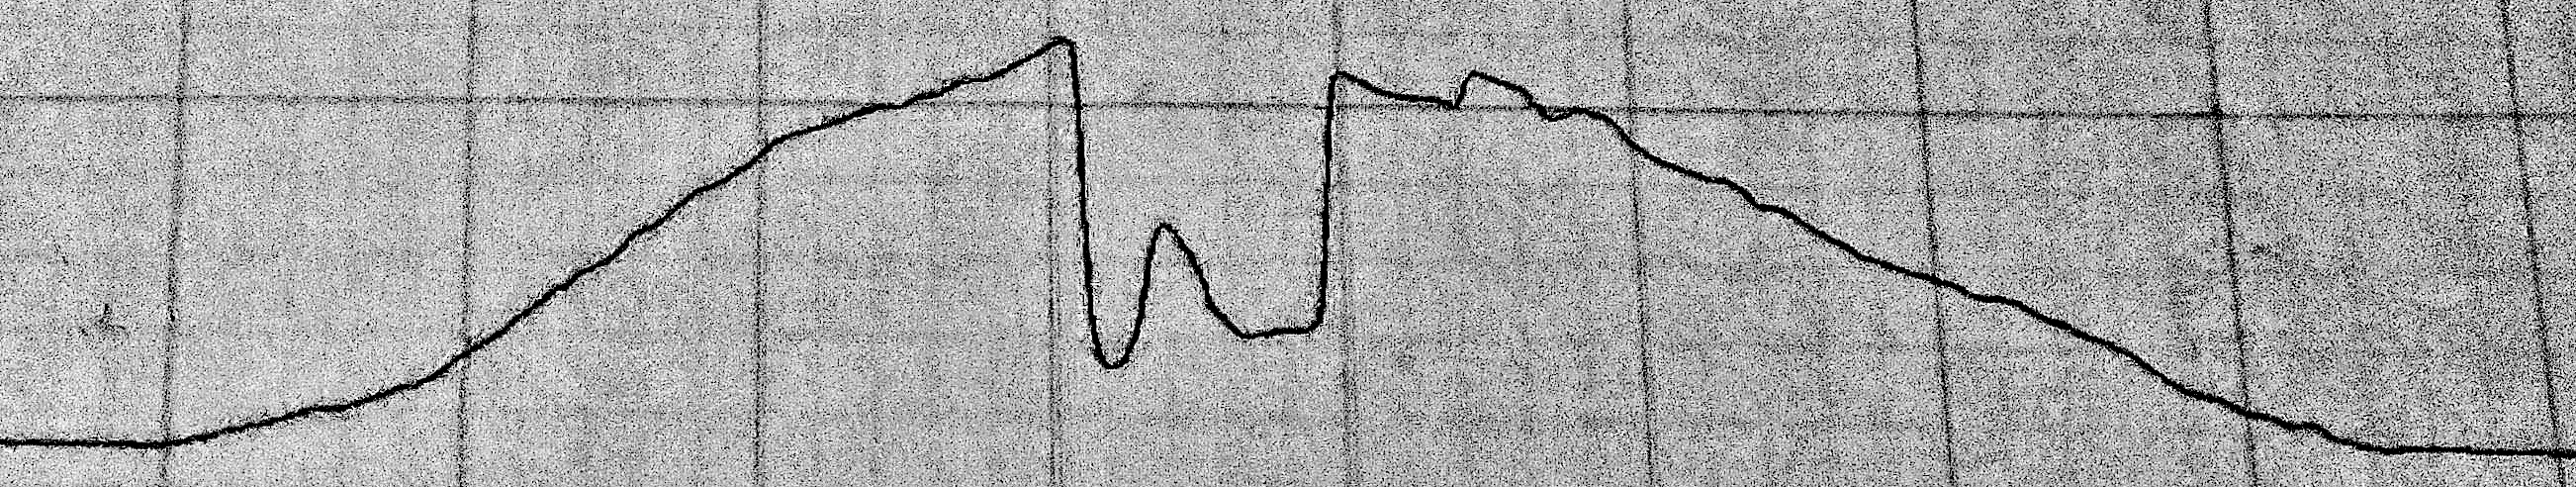
\includegraphics[width=\textwidth]{assets/images/spektrum_600L.png}
        \caption{Tatsächliches Signal}
    \end{figure}

\end{frame}

\subsection{Arduino}
\begin{frame}
    \frametitle{IR-Spektrometer}
    \framesubtitle{Arduino}

\begin{semiverbatim}
rpm = 60

stepsPerRev = 200

range = 150

rangePerRev = 20

interval = 1


stepsPerInterval = (interval / rangePerRev) * stepsPerRev
intervalAmount = range / interval
\end{semiverbatim}
\end{frame}

\begin{frame}
    \frametitle{IR-Spektrometer}
    \framesubtitle{Arduino}

\begin{semiverbatim}
for (int i = 0; i < intervalAmount; i++) \{


    stepper.step(stepsPerInterval)


    Serial.println(String(i * measurementInterval) + ``   '' + String(analogRead(A0)))


\}
\end{semiverbatim}
\end{frame}

\begin{frame}
    \frametitle{IR-Spektrometer}
    \framesubtitle{Arduino}
    \begin{figure}
        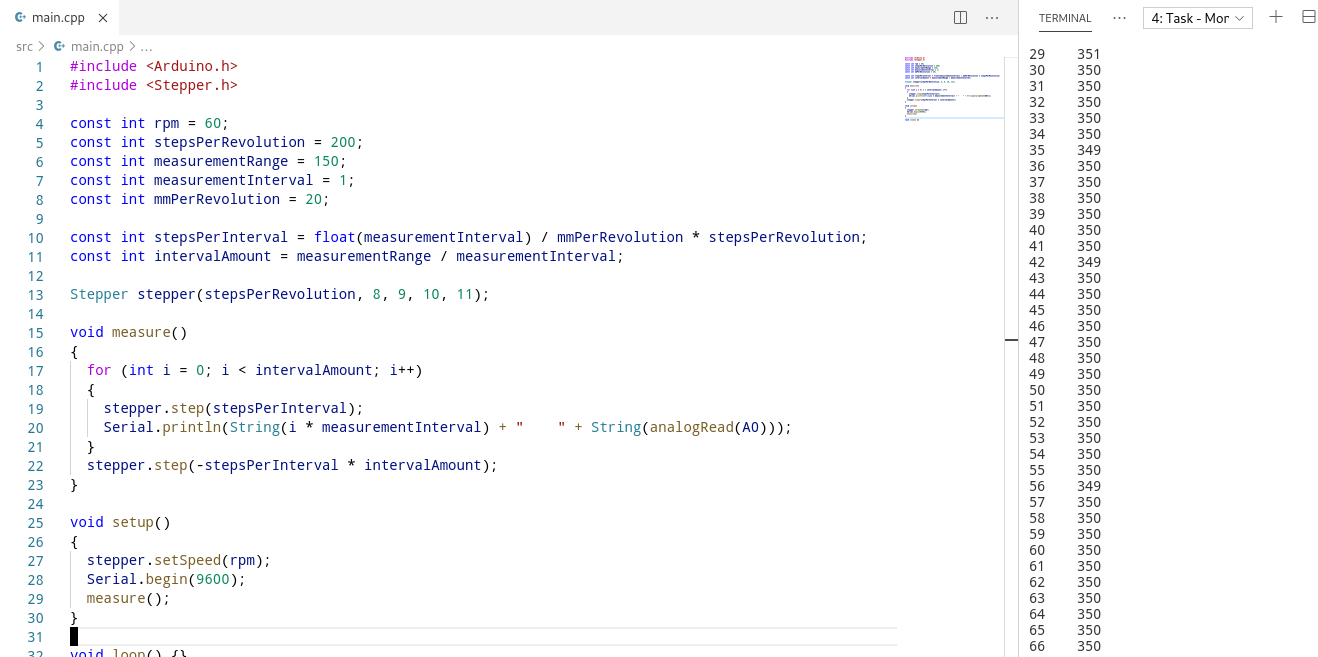
\includegraphics[width=\textwidth,height=\textheight,keepaspectratio]{assets/images/platformio.png}
    \end{figure}
\end{frame}